\subsection{Mobility}
As \ues{} traverse the \xcloud{} network, the service(s) they subscribe to will migrate accordingly to accommodate the changing distribution of \ues{} in the network. The 2-dimensional, multi modal, mobility model detailed in \cite{bettstetter2001smooth} provides us with a uniform distribution of users, with a realistic rate of mobility, see Figure \ref{fig:mobility_distribution}.

\begin{figure}[tb]
	\centering
	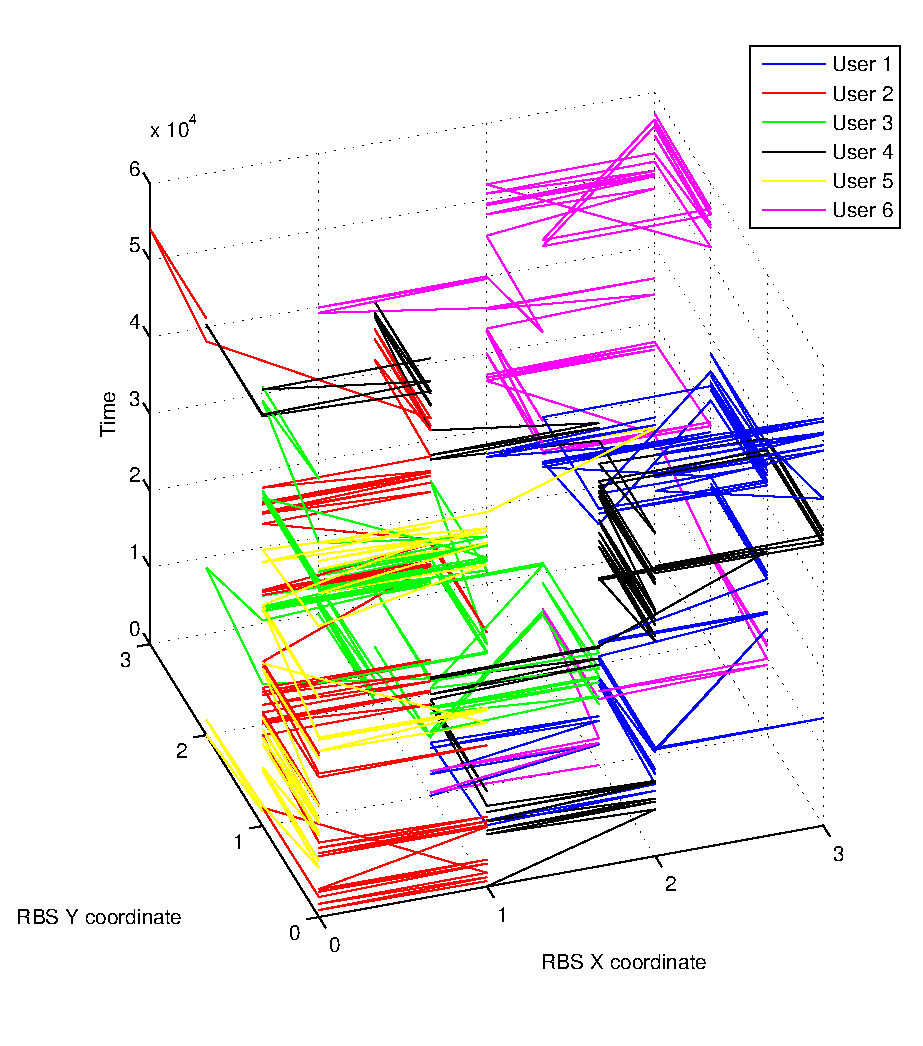
\includegraphics[width=\linewidth]{user_mobility.eps} 
	\caption{\Ue mobility between \rbs{} over time}
	\label{fig:mobility_distribution}
\end{figure}

The model defines the fundamental timing and mobility properties of \ue{} movement, such as the speed, acceleration, and direction the \ue{} is moving in, as well as for how long and when in time to turn next. 